\section{Machine Code Translation}
\label{chap:QEMU_Translation}

As mentioned, QEMU at its core employs binary translation technology, allowing 
it to interpret and execute machine code compiled for one type of CPU on a 
completely different CPU. A typical binary translation converts the guest CPU's 
(also known as virtual CPU or vCPU) entire binary file into the host CPU's binary file 
using some method, and then executes the converted binary on the host CPU. 
However, this approach presents a significant problem, any modifications made to the 
guest program require, once again, a complete binary conversion. This wouldn't be 
a problem for small programs, but it is for larger ones. Longer conversion times may 
be acceptable for large guest programs if the conversion only needs to be done once. 
But, when frequent modifications to the guest program is need, like in embedded 
software development, this approach becomes impractical.

QEMU solves this problem by not implementing a traditional translation 
technology, instead use dynamic binary translation (DBT). This type of translation 
does not convert the entire vCPU program at once. it only converts the necessary parts 
of the program and executes them. For example, when booting a guest OS, only 
the parts required for booting are converted and executed. To be more specific, 
QEMU advances the program counter for the vCPU step by step, converting one 
vCPU instruction into one or more host CPU instructions and executing them, 
then advancing the program counter again, converting, executing, and repeating 
this process. With this method, there is no need to convert the parts that are 
not executed.

The inefficiency of translating the entire program binary from the vCPU is evident. 
However, translating and executing only one guest instruction at a time 
incurred a considerable time overhead. This is due to context management. 
QEMU is a regular program running on the host CPU, so to execute the instructions 
translated from the vCPU, it first needs to save the state of the host CPU's registers and 
memory context. Furthermore, once the translated instruction finishes executing, 
the saved state of the host CPU must be restored. Because of this inefficiency, 
DBT parses a short chunks of code, translates it, and caches the resulting sequence. 
This way, code is only translated as it is discovered and when possible, and branch 
instructions are configured to point to code that has already been translated and saved.

%==== TCG ====%
\subsubsection{Tiny Code Generator}
\label{chap:QEMU_TCG}

QEMU's DBT takes the named of the Tiny Code Generator (TCG), and the basic 
code fragments it analyzes are called Translation Blocks (TB). These TBs are 
defined by jump instructions at machine code branch points and emulated hardware 
accesses (peripheral accesses) as boundaries\cite{QemuTCGOpsDevel} \cite{QemuTCGDirectBlockChaining}. 

The figure \ref{fig:TCG} illustrates the overall TCG architecture and workflow. Where the 
"Target Machine Code" corresponds to a TB, the blue part of the diagram represents 
the TCG, and the last block represent the "Host Machine Code".

\begin{figure}
    \centering
%    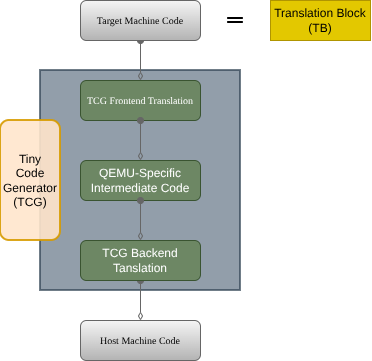
\includegraphics[width=0.5\textwidth]{Resources/Draw/TCG.png}
    \caption{Tiny Code Generator}
    \label{fig:TCG}
\end{figure}

As can be seen in \ref{fig:TCG}, the TCG operates through a two-phase translation 
process. In the first phase, the front-end translation part of the TCG, decodes 
the guest instructions into QEMU-specific intermediate representation (IR). 
Conceptually, this IR it is like an assembly language designed specifically for QEMU's 
compilation infrastructure. In the second phase, the back-end translation part of 
the TCG converts this intermediate representation into native host machine code, 
which is then directly executable on the host processor\cite{QemuTCGFrontendOps}\cite{QemuTCGBackendOps}.

The separation of front-end and back-end translation was due it provides 
significant advantages for QEMU's scalability. In order to support a new guest CPU 
architecture, developers need only implement a new front-end translator, while the 
back-end translation logic remains unchanged. Conversely, supporting QEMU on a 
new host architecture requires only back-end development, leaving guest architecture 
support unaffected. This modularity is the primary reason for QEMU's scalability 
across diverse hardware platforms and CPU architectures.

%==== Host Code ====%
\subsubsection{Execution Of Host Code}
\label{chap:QEMU_Host}
